\documentclass[12pt]{article}
\usepackage{iftex}
\usepackage{graphicx}
\usepackage{enumitem}
\usepackage{hyperref}
\usepackage[style=apa, backend=biber]{biblatex}
\addbibresource{phd_bombus.bib}
\setcounter{maxnames}{20}
\setcounter{minnames}{1}
\usepackage{color}
\usepackage{amsmath}
\usepackage{amssymb}
\usepackage[export]{adjustbox}
\usepackage{verbatim}
\usepackage{mathpazo}
\usepackage{setspace}
\usepackage{multirow}
\usepackage{lscape}
\usepackage{fancyhdr}
\usepackage[normalem]{ulem}
\usepackage{rotating}
\usepackage{chngcntr}
\usepackage{float}
\usepackage[parfill]{parskip}
\usepackage[tiny,compact]{titlesec}
\usepackage{longtable}
\usepackage{textcomp}
\usepackage{rotating}
\usepackage{xr}
\usepackage{caption}
\usepackage{siunitx}
\usepackage[T1]{fontenc}
\usepackage{gensymb}
\sisetup{round-mode=places, round-precision=2, detect-all}

\newcommand{\flagged}[1] {
  \textcolor{blue}{#1}
}

\hypersetup{colorlinks=true, linkcolor=black, citecolor=black}
\RequirePackage{lineno}

\renewcommand{\thefigure}{A\arabic{figure}}  % Prefix figures with "S"
\setcounter{figure}{0}  % Reset figure counter
\renewcommand{\thetable}{A\arabic{table}}
\setcounter{table}{0}
\setcounter{section}{0}

\def\title{Appendix 1 -- Population Genetics and Colony Assignments}



\begin{document}
\begin{center}
  {\large \title \par}
\end{center}\par

\section{Assessing locus $F_{is}$, $F_{st}$ and linkage disequilibrium}

\begin{figure}[H]
    \centering
    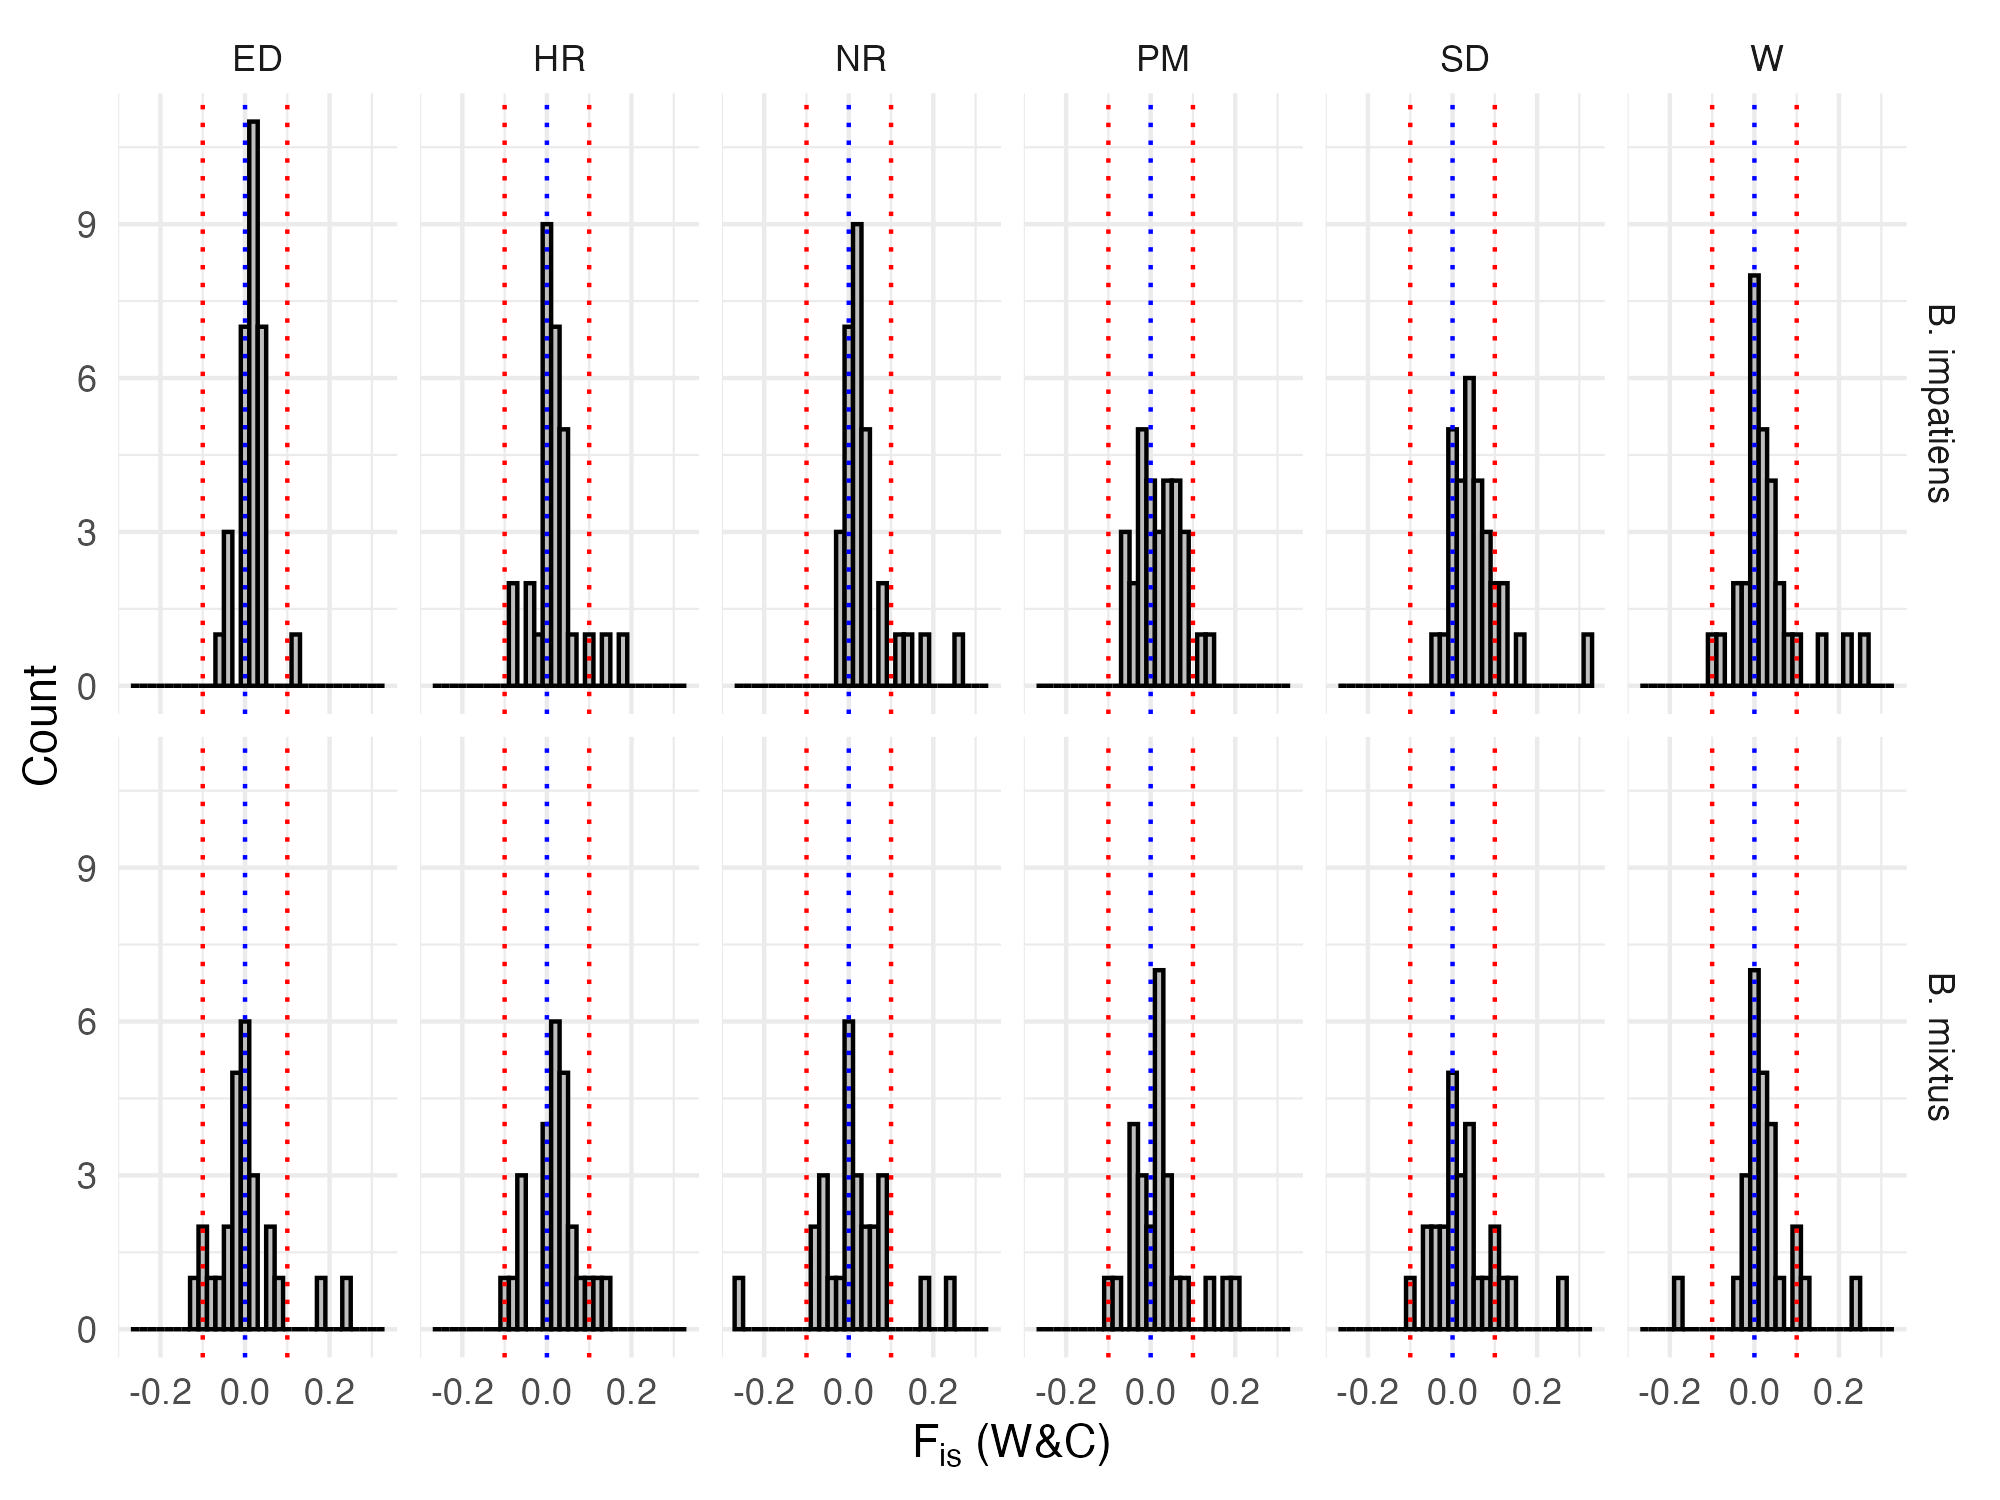
\includegraphics[width=\linewidth]{appendix_figures/Fis.jpg}
    \caption{Estimates of $F_{is}$ for each locus in each subpopulation. Estimates from 2022 and 2023 were calculated separately but are shown together for each site x species combination. Blue dotted lines indicates $F_{is} = 0$ and red dotted lines indicate $F_{is} = \pm 0.1$.}
    \label{fig:Fis}
\end{figure}


\begin{figure}[H]
    \centering
    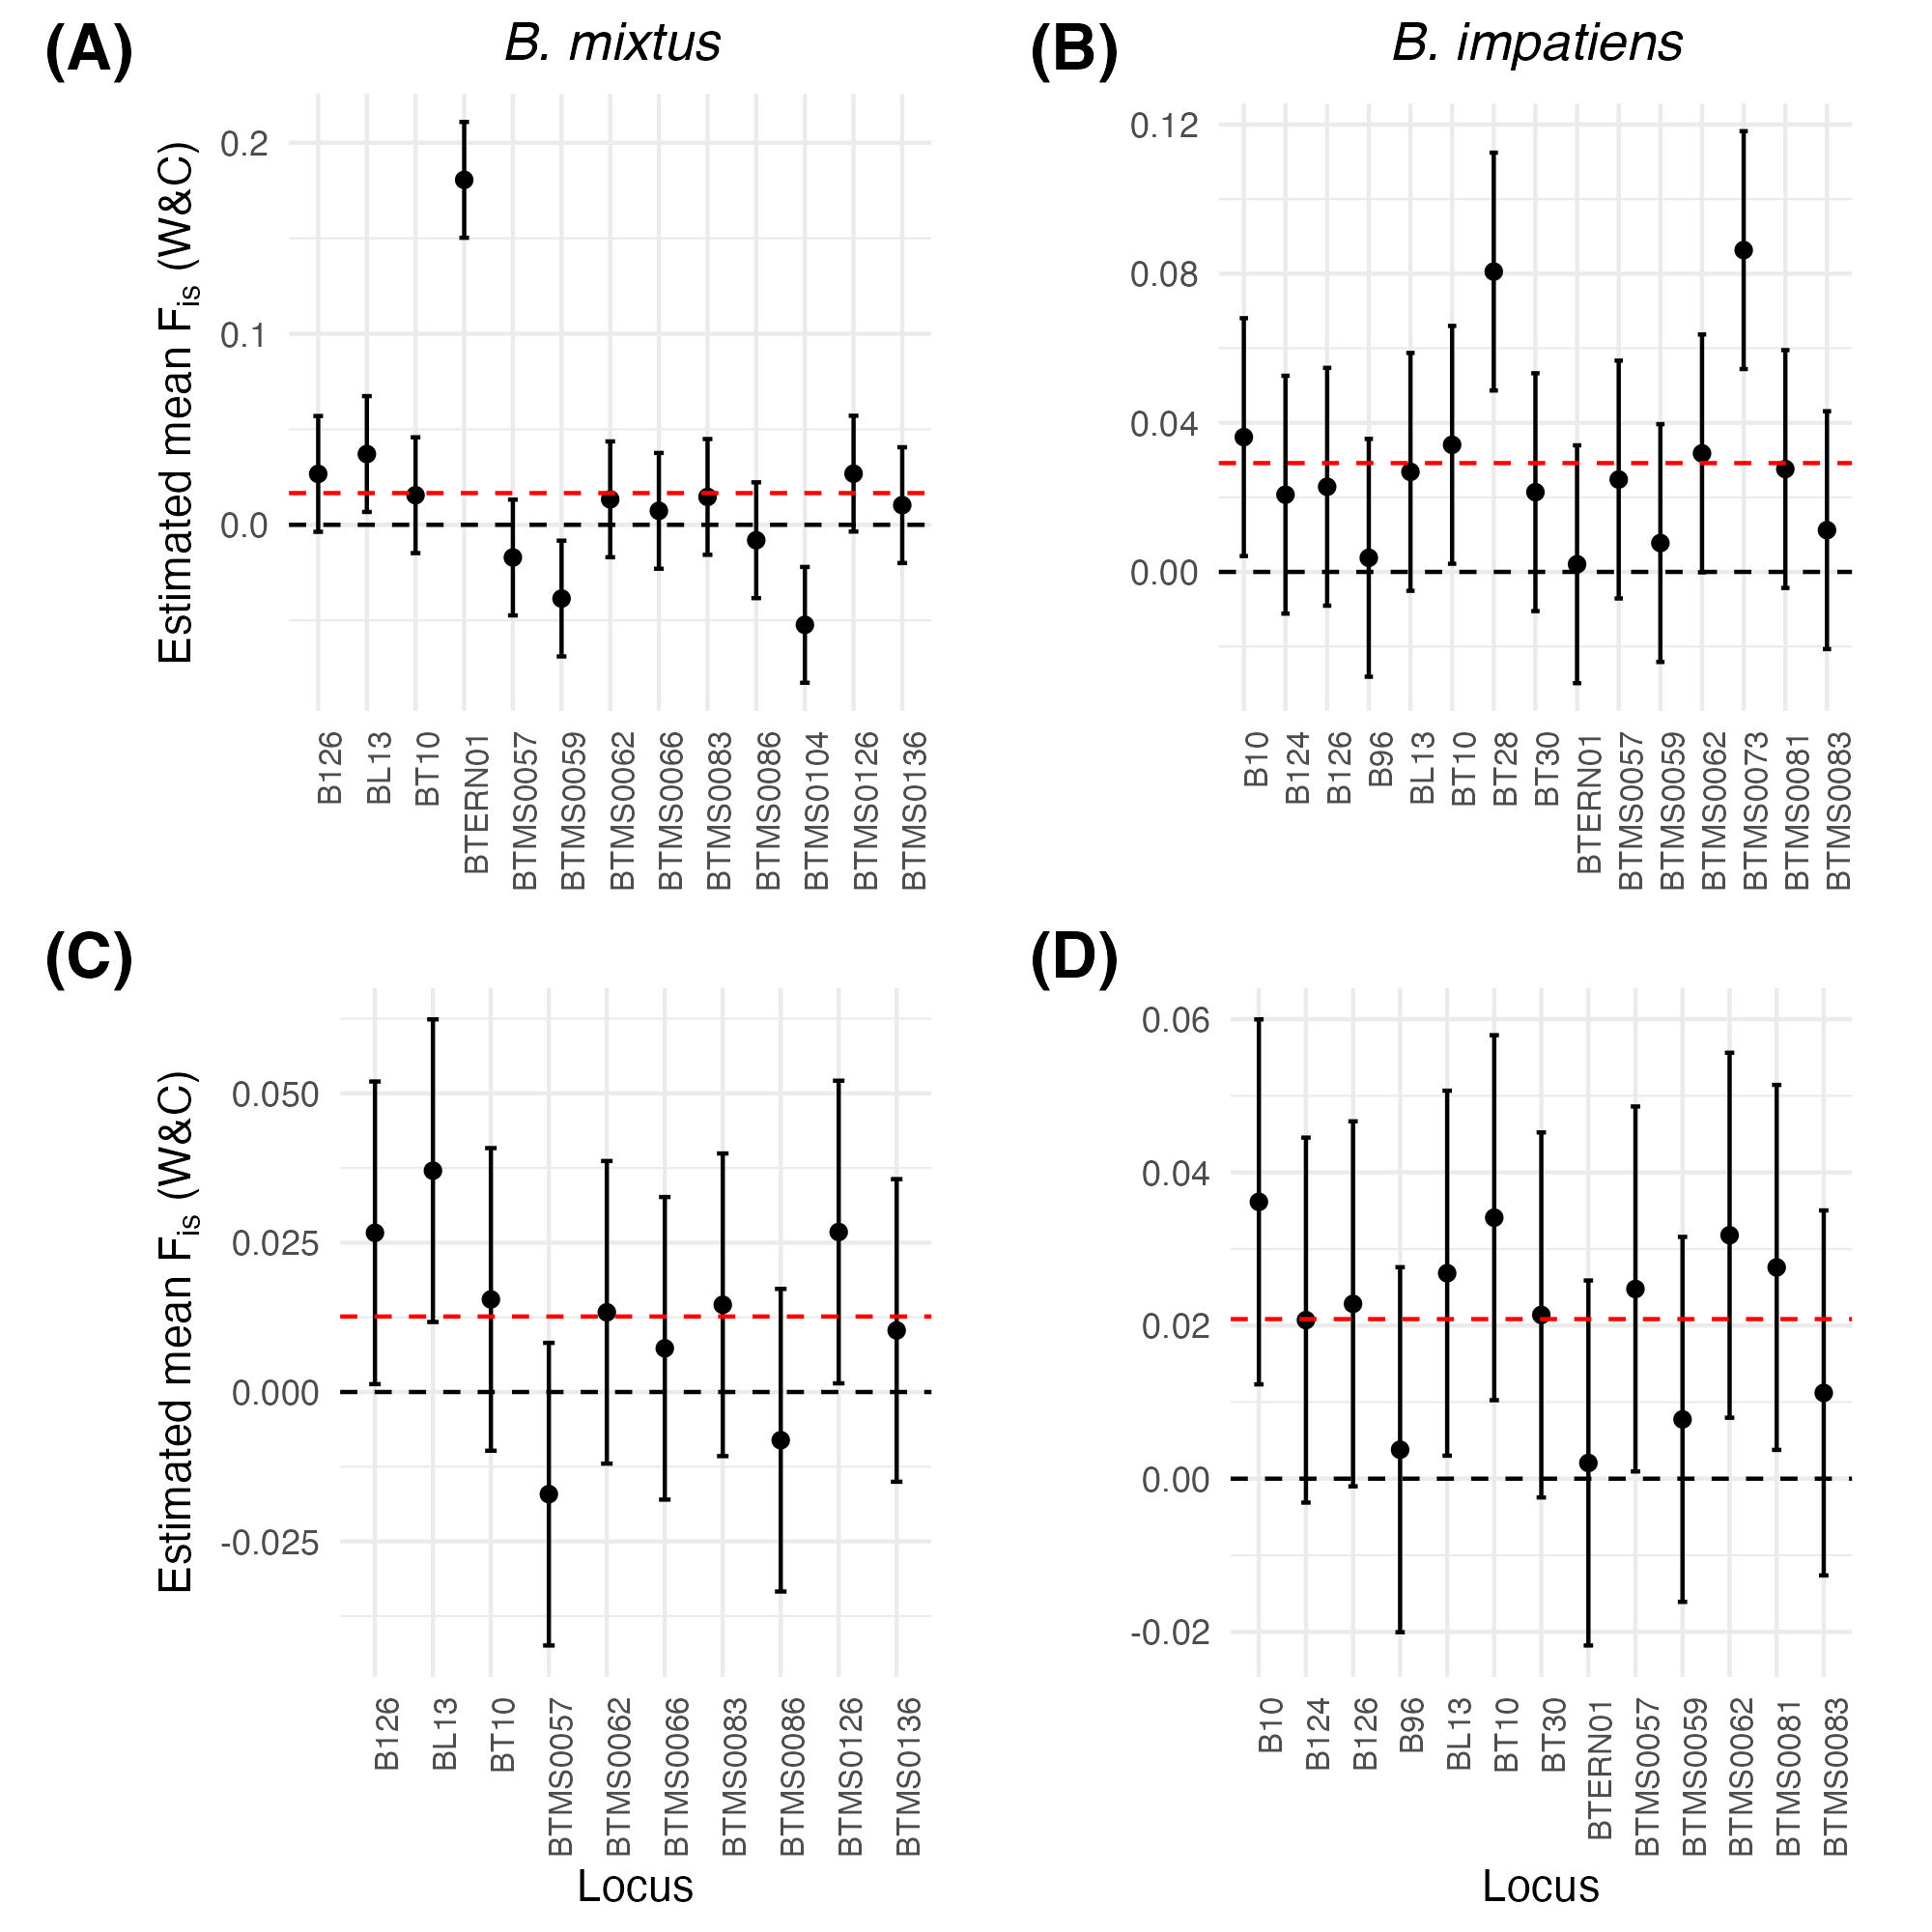
\includegraphics[width=\linewidth]{appendix_figures/marginalmeans.jpg}
    \caption{Locus-specific $F_{is}$ marginal means. A) \emph{B. mixtus} all loci; B) \emph{B. impatiens} all loci; C) \emph{B. mixtus} loci following iterative removal of loci which differed significantly from global mean $F_{is}$; D) \emph{B. impatiens} loci following iterative removal of loci which differed significantly from global mean $F_{is}$. Dashed black line denotes $F_{is} = 0$, dashed red line denotes global mean $F_{is}$ for each species.}
    \label{fig:marginalmeans}
\end{figure}


\begin{figure}[H]
    \centering
    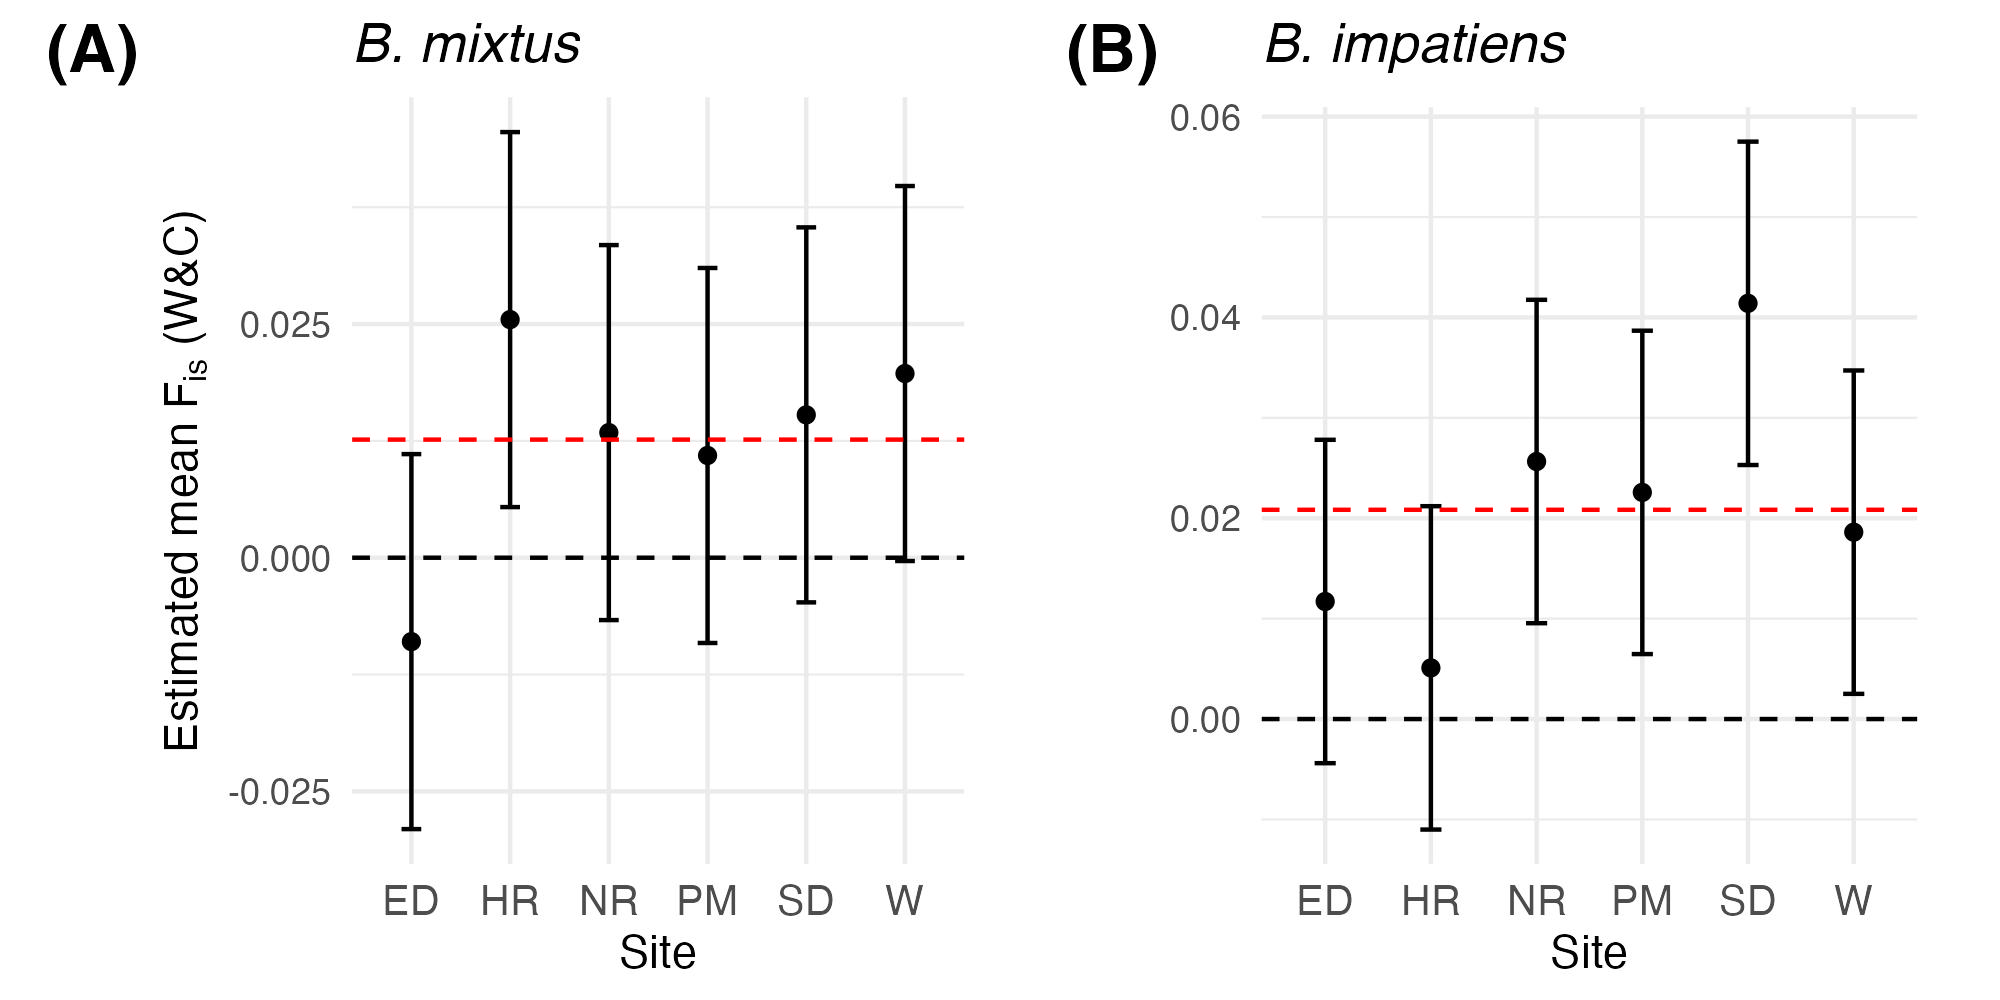
\includegraphics[width=\linewidth]{appendix_figures/siteFis.jpg}
    \caption{Site-specific $F_{is}$ marginal means following removal of low-quality loci for A) \emph{B. mixtus} and B) \emph{B. impatiens}. Dashed black line denotes $F_{is} = 0$, dashed red line denotes global mean $F_{is}$ for each species.}
    \label{fig:siteFis}
\end{figure}


\section{Testing COLONY on simulated data}
To test the informativeness of our genetic loci and to validate the accuracy of COLONY2.0 \parencite{jonesCOLONYProgramParentage2010} for accurately detecting siblingships amongst our samples, we performed simulations using realistic family size distributions and the allelic frequencies present in our real data.

We approached this simulations with four objectives:

(i) To determine false positive and false negative siblingship assignment rates, given the informativeness of our microsatellite datasets, 

(ii) To inform an appropriate strategy (probability threshold, number of runs of the software) for maintaining or rejecting each sib-pair;

(iii) To select suitable software parameters, and in particular to evaluate the usefulness of siblingship size priors and exclusion of across-site siblingships for reducing false positive rates as sample size increases;

(iv) To assess whether modelling female polygamy would improve family reconstruction in the case of sibling genotypes simulated under varying rates of multiple paternity.

\subsection{Simulation strategy}
We simulated siblingships following \textcite{popeInferringForagingRanges2017}. In brief, we began by simulating six 5 x 5 trapping grids within a single raster surface, and then placed colonies uniformly at random throughout the raster. We sampled individuals from colonies $i \in \mathbb{C}$ captured at traps $k \in \mathbb{K}$ from the joint distribution $\Pr(s, c \mid s \in \kappa)$, where ${s,c}$ are the indices of a random visitation event of an individual from colony $c$ to grid cell $s$, where $s$ belongs to $j \in \mathbb{J}$, the set of all grid cells in the raster. 

To do this, we first sampled a trap $k \in \mathbb{K}$ from $\Pr(s=k \mid s \in \kappa)$, which is defined as:

\[
\Pr(s = k \mid s \in \kappa) \;=\; \frac{\Pr(s = k)}{\Pr(s \in \kappa)}
\]

where

\[
\Pr(s = k) \;=\; \sum_{i \in C} \Pr(s = k \mid c = i)\,\Pr(c = i)
\]

and

\[
\Pr(s \in \kappa) \;=\; \sum_{i \in C} \Pr(s \in \kappa \mid c = i)\,\Pr(c = i)
                  \;=\; \sum_{k \in \kappa} \Pr(s = k \mid c = i)\,\Pr(c = i)
\]

We define the foraging kernel of workers from colony i as:

\[
\Pr(s = k \mid c = i)
\;=\; 
\frac{\lambda_i(k)}{\sum_{j \in J} \lambda_i(j)}
\]

where $ln(\lambda_i(j)) = \frac{- \lVert x_j - \delta_i \rVert}{\rho}$, where $x_j$ are the spatial coordinates of any grid cell in the raster, and $\delta_i$ are the spatial coordinates of colony $i$ (e.g., a symmetrical, exponential decay of visitation intensity as a function of distance from the colony location).





% FIRST the stuff I haven't done yet -- prob threshold vs more runs -- determine and appropriate probability threshold!


% SECOND sample size effects -- do exclusion tables help?
% --> rerun some of these but without sibship size prior? for below?

% Multiple paternity results
\section{Observing colonymates at multiple sites}


\end{document}